\documentclass[conference]{IEEEtran}
\IEEEoverridecommandlockouts

\usepackage[T1]{fontenc}
\usepackage{cite}
\usepackage{amsmath,amssymb}
\usepackage{graphicx}
\usepackage{booktabs}
\usepackage{multirow}
\usepackage{url}
\usepackage[hidelinks]{hyperref}
\usepackage{balance}
\usepackage{tikz}
\usetikzlibrary{arrows.meta,positioning,fit}
\newcommand{\method}[1]{\textsc{#1}}

\graphicspath{{figures/}}
\setlength{\textfloatsep}{6pt plus 1pt minus 2pt}
\setlength{\floatsep}{6pt plus 1pt minus 2pt}
\setlength{\dbltextfloatsep}{6pt plus 1pt minus 2pt}
\setlength{\dblfloatsep}{6pt plus 1pt minus 2pt}
\setlength{\abovecaptionskip}{2pt}
\setlength{\belowcaptionskip}{0pt}

\begin{document}

\title{A Deployment Study of Identity-Gated\\Drone Gesture Control}

\author{Diyari Mohammed Salih$^{1}$,
        Ilyes Chaabeni$^{1}$,
        and Na\"{\i}ma A\"{\i}t Oufroukh$^{2}$%
\thanks{$^{1}$M2 Smart Aerospace and Autonomous Systems,
Universit\'e Paris-Saclay, \'Evry, France.}%
\thanks{$^{2}$IBISC Laboratory, Universit\'e Paris-Saclay, \'Evry, France.}%
\thanks{E-mails: diyari.m.salih@gmail.com,
chaabeni.ilyes2002@gmail.com,
naima.aitoufroukh@univ-evry.fr.}%
}

\maketitle

\begin{abstract}
Vision-based gesture control accepts commands from any hand in the camera field
of view, which is unsafe in shared indoor spaces. This paper presents
\method{IGate}, an identity-gated control stack for the DJI Tello EDU in which
gesture and tracking commands are admitted only while an enrolled operator is
verified, arbitration is performed by a deterministic hierarchical state machine,
and a local language model is confined to post-hoc explanation. The contribution
is how it is evaluated: every component is characterised both by the metric
conventionally reported for it and by the rate it achieves through the aircraft's
own video pipeline, over per-frame logs dense enough to reconstruct any trial
after the fact. Across 270 logged trials over 43 instrumented runs, 149 of them
flown, the two disagree systematically. Gesture accuracy is 0.997 under a
within-session random split, 0.910 held out across four capture sessions and
0.783 through the aircraft's optics; face verification reports a 0.32\% offline
equal error rate against 19.3\% in flight, a gap that separates into the cost of
the imagery and the cost of an operating threshold three times the equal-error
point. A fourth capture session disentangles background from illumination, though at
two against four ordered pairs the two factors do not separate; a post-hoc
analysis instead finds that coverage of the test session's hand-scale range by
the training session's predicts transfer better than either ($r=0.76$ against
0.30 and $-0.09$). The stack carries two gesture classifiers decoding different vocabularies, and
both are flown under an identical hover-locked cue at matched standoff: the
RBF-SVM reaches 0.850 in flight and the geometric rule 0.651, with 82\% of that
gap on the depth channel. Expressing depth as a static pose rather than a motion
removes the motion cue's pathology outright, taking FORWARD from 0.000 to 0.777,
and in doing so exposes a second and independent problem: the BACK pose reaches
only 0.336 because it sits inside the landmark estimator's noise floor against
LEFT and RIGHT, three poses being distinguished by a single extended digit that
the estimator does not reliably resolve. All instrumentation, logs
and a script that rederives every number reported here are released.
\end{abstract}

\begin{IEEEkeywords}
human-drone interaction, gesture control, face verification, deployment
evaluation, unmanned aerial vehicles, mode arbitration
\end{IEEEkeywords}

% =====================================================================
\section{Introduction}

Small indoor drones are increasingly operated through vision-based gesture
interfaces, which remove the physical controller and lower the barrier for novice
users. A camera-based recogniser, however, responds to whichever hand enters the
field of view, so in a shared indoor space it admits commands from bystanders;
prior gesture-controlled UAV systems generally treat any detected hand as a valid
operator. Predictable interaction therefore requires two rarely combined
capabilities: identity-aware authorization, so that only an enrolled operator's
commands are honoured, and deterministic arbitration between teleoperation,
tracking and safety behaviours, so that mode transitions are explicit and
traceable rather than emergent consequences of noisy perception.

This paper presents \method{IGate}, an identity-gated gesture control stack for
the DJI Tello EDU, and evaluates it in flight. The design is conventional in its
parts: MediaPipe landmarks, an RBF-SVM gesture classifier, an ArcFace-trained
face embedding, and a hierarchical state machine. The contribution lies in the
evaluation. Each component of \method{IGate} is characterised both by the offline
metric conventionally reported for it and by the rate it achieves through the
aircraft's own video pipeline, and for every component that measurement is
taken in flight, the cued captures holding the aircraft on station so that a
sustained command does not carry it out of the room
(Section~\ref{sec:inflight}). The size of the gap is not uniform across the
stack: it is large where a component depends on image quality, the identity gate
losing a factor of 23 in false rejection to the aircraft's imagery at a fixed
threshold, and small where it depends on evaluation protocol, gesture accuracy
moving from 0.997 to 0.850 almost entirely through the choice of split. The
paper argues that the operational figure is the one a deployed system should be
judged by, and that which of the two causes dominates is itself a result.

Diagnosing which of these is at work requires per-frame logging dense enough to
reconstruct a trial's internal state after the fact, released here with the
system.

The contributions of this paper are as follows:

\begin{itemize}
\item \method{IGate}, an identity-gated human-drone interaction stack in which
      gesture and tracking commands are filtered by session-level face
      verification and arbitrated by a deterministic hierarchical state machine,
      with a local language model excluded from actuation.
\item A three-protocol evaluation of the gesture classifier giving 0.997, 0.910
      and 0.783, a hover-locked in-flight comparison of both deployed
      classifiers at matched standoff giving 0.850 against 0.651, and a
      four-session design that does not resolve background from illumination but
      identifies hand-scale coverage as the better predictor of transfer.
\item An operational characterisation of the identity gate, comprising false
      rejection rate through the aircraft video pipeline and an authorization
      envelope in apparent face size, reported against the offline equal error
      rate of the same model.
\item Characterisation of six deployment behaviours that appear only in flight,
      three of them corrected and reported with paired measurements, together with
      in-flight ablations of the identity gate and of authorization hysteresis.
\end{itemize}

Every quantitative claim in this paper is rederived from the released logs by an
accompanying audit script, which reports any figure it cannot reproduce; the
tables and figures are generated by the same pipeline.

\section{Related Work}
\label{sec:related}

\subsection{Gesture Control for Unmanned Aerial Vehicles}

Vision-based hand gesture recognition is long established in human-computer
interaction, with persistent difficulties around variability and
robustness~\cite{wachs2011,foteinos2025hgrreview}. This work uses MediaPipe Hands~\cite{zhang2020},
whose compact 21-landmark representation suits low-latency host-side perception.
Six of the seven classes are static configurations and need no temporal model.
The two depth classes are the exception in the deployed path, where they are
derived from frame-to-frame change rather than from a pose, and
Section~\ref{sec:depth} reports what that choice costs.

Gesture control has been demonstrated on UAVs across platforms and scales:
Latif \emph{et al.}~\cite{latif2022} control a small quadrotor from a
TensorFlow gesture detector, reporting 95.7\% detection accuracy;
HGIC~\cite{hu2024hgic} extends the approach to multi-UAV
operation and reports reduced task-completion time for novice operators, and
Taylor \emph{et al.}~\cite{taylor2025} pair gesture piloting with obstacle
avoidance, and Abdalla and Baidya~\cite{abdalla2025edge} offload the same
landmark pipeline to an edge server to close the control loop in real time.
Dedicated datasets exist for the task, notably
\mbox{UAV-GESTURE}~\cite{perera2018uavgesture}, which records thirteen
navigation gestures for outdoor control. These systems establish that
landmark-based gesture control is practical on low-cost hardware; they
characterise their classifiers by held-out accuracy on such datasets and
describe system behaviour qualitatively.

\subsection{Identity-Aware Authorization}

Embedding-based face verification separates identities effectively under
unconstrained conditions~\cite{schroff2015,deng2019} and is conventionally
characterised by equal error rate on curated still-image
benchmarks~\cite{huang2008}. That characterisation is known to travel poorly:
Cheng \emph{et al.}~\cite{cheng2018survface} report a large drop between
benchmark figures and native surveillance imagery, and argue that the shortfall
is a property of the imagery rather than of the embedding.
Section~\ref{sec:identity} measures the same effect through an aircraft's video
link and separates it from the cost of the operating point. Seidu and Lawal~\cite{seidu2024} apply it as an
authorization gate, combining facial authentication with gesture control on a DJI
Tello; that system is the closest published work to \method{IGate}, and its
evaluation likewise addresses component accuracy rather than the rate at which
the composed gate admits or refuses the operator in flight.

\subsection{Evaluation Protocol and Learned Components}

The protocol concern raised here has a direct precedent. Varga~\cite{varga2026}
critiques a published UAV gesture-recognition result on the grounds that
frame-level random train-test splitting mixes samples from the same subject
across both partitions, so the resulting near-perfect accuracy does not measure
generalisation, and argues for subject-independent partitioning. This work
reaches a consistent conclusion from session-independent partitioning, which
removes a different leakage axis from the one Varga identifies: all four sessions
record a single operator, so every figure reported here is within-subject and is
an upper bound on cross-subject performance. It additionally decomposes capture
domain, separating background from illumination
with a fourth session, while noting that neither fully accounts for the transfer
asymmetries (Section~\ref{sec:gesture}). Separately, language models have been grounded in
robot action through affordance value functions~\cite{ahn2022saycan}, and the
risk that hallucination propagates into physical behaviour has motivated
guardrail architectures~\cite{ravichandran2025}; \method{IGate} excludes the
model from actuation entirely (Section~\ref{sec:llm}).

\begin{table}[t]
\caption{Positioning against representative gesture-controlled UAV systems.
``Operational'' means measured through the aircraft's own video pipeline.
$^{\dagger}$In-flight gesture accuracy and in-flight false rejection.}
\label{tab:related}
\centering
\footnotesize
\setlength{\tabcolsep}{4pt}
\renewcommand{\arraystretch}{1.02}
\begin{tabular}{@{}lcccc@{}}
\toprule
& Identity & Explicit & Cross-sess. & Operational \\
& gate & arbitration & eval. & rates$^{\dagger}$ \\
\midrule
Latif \emph{et al.}~\cite{latif2022}      & --  & --  & --  & -- \\
HGIC~\cite{hu2024hgic}                    & --  & yes & --  & -- \\
Taylor \emph{et al.}~\cite{taylor2025}    & --  & yes & --  & -- \\
Seidu \& Lawal~\cite{seidu2024}           & yes & --  & --  & -- \\
Varga~\cite{varga2026}                    & --  & --  & yes & -- \\
\midrule
This work                                 & yes & yes & yes & 0.850\,/\,19.3\% \\
\bottomrule
\end{tabular}
\end{table}


\section{Proposed Method: \method{IGate}}
\label{sec:system}

\subsection{Architecture and Platform}
\label{sec:arch}

\begin{figure*}[t]
\centering
\resizebox{\textwidth}{!}{% Generated by tello_gesture_py/src/gestures/build_design_figures.py
% Do not edit: every value here is read from the deployed configuration.

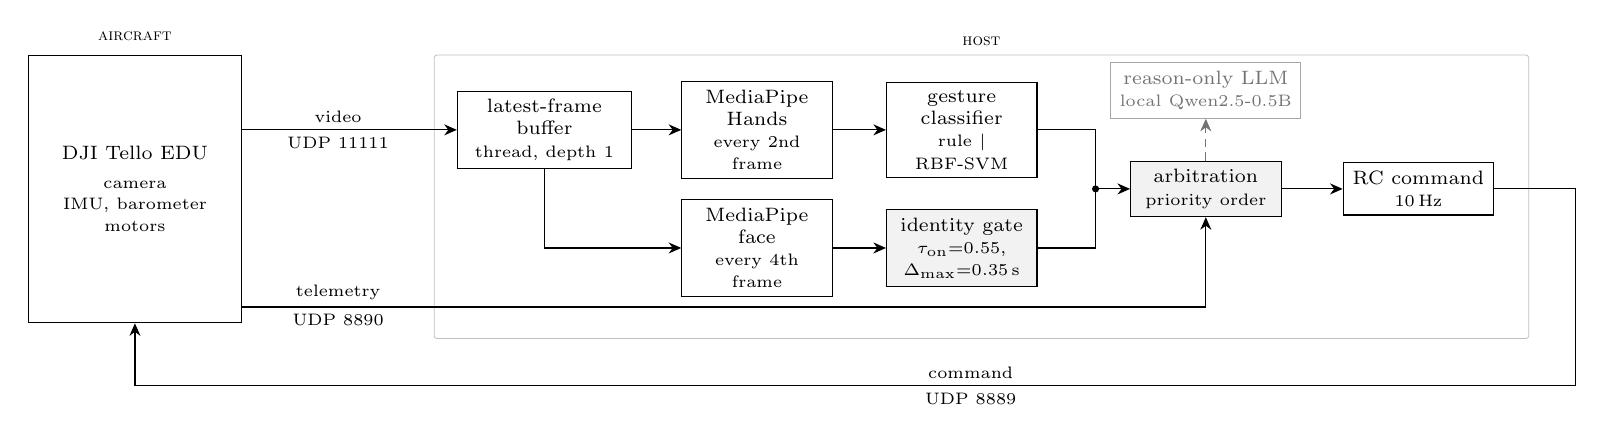
\begin{tikzpicture}[x=1mm,y=1mm]

\tikzset{
  blk/.style   = {draw, line width=0.4pt, inner sep=3pt, align=center,
                  minimum height=6.5mm, font=\scriptsize},
  wide/.style  = {blk, text width=20mm},
  narrow/.style= {blk, text width=17mm},
  gate/.style  = {wide, fill=black!4},
  aux/.style   = {wide, draw=black!35, text=black!55},
  flow/.style  = {-{Stealth[length=1.6mm,width=1.4mm]}, line width=0.4pt},
  aside/.style = {flow, densely dashed, draw=black!55},
  lbl/.style   = {font=\fontsize{6}{7}\selectfont, inner sep=1.5pt},
  grp/.style   = {draw=black!25, line width=0.3pt, rounded corners=1pt,
                  inner sep=0pt},
}


\node[blk, text width=25mm, minimum height=34mm] (air) at (0,0) {DJI Tello EDU\\[3pt]\fontsize{6}{7.5}\selectfont camera\\ IMU, barometer\\ motors};
\node[lbl, above=1.2mm of air] {\textsc{aircraft}};
\node[grp, fit={(38,-19) (177,17)}] (host) {};
\node[lbl, above=0.6mm of host.north] {\textsc{host}};
\node[wide] (buf) at (52,7.5) {latest-frame buffer\\\fontsize{6}{7}\selectfont thread, depth 1};
\node[narrow] (hand) at (79,7.5) {MediaPipe Hands\\\fontsize{6}{7}\selectfont every 2nd frame};
\node[narrow] (face) at (79,-7.5) {MediaPipe face\\\fontsize{6}{7}\selectfont every 4th frame};
\node[narrow] (clf) at (105,7.5) {gesture classifier\\\fontsize{6}{7}\selectfont rule \textbar{} RBF-SVM};
\node[narrow, fill=black!5] (gate) at (105,-7.5) {identity gate\\\fontsize{6}{7}\selectfont $\tau_{\mathrm{on}}{=}0.55$, $\Delta_{\max}{=}0.35$\,s};
\node[narrow, fill=black!5] (fsm) at (136,0) {arbitration\\\fontsize{6}{7}\selectfont priority order};
\node[narrow] (rc) at (163,0) {RC command\\\fontsize{6}{7}\selectfont 10\,Hz};
\node[aux, text width=22mm] (llm) at (136,12.5) {reason-only LLM\\\fontsize{6}{7}\selectfont local Qwen2.5-0.5B};
\draw[flow] (air.east |- buf) -- (buf.west);
\node[lbl, above=0.3mm] at (25.80,7.5) {video};
\node[lbl, below=0.3mm] at (25.80,7.5) {UDP 11111};
\draw[flow] (buf.east) -- (hand.west);
\draw[flow] (hand.east) -- (clf.west);
\draw[flow] (buf.south) -- (52,-7.5) -- (face.west);
\draw[flow] (face.east) -- (gate.west);
\draw[line width=0.4pt] (clf.east) -- (122,7.5);
\draw[line width=0.4pt] (gate.east) -- (122,-7.5);
\draw[line width=0.4pt] (122,7.5) -- (122,-7.5);
\draw[flow] (122,0) -- (fsm.west);
\fill (122,0) circle (0.45);
\draw[flow] (fsm.east) -- (rc.west);
\draw[aside] (fsm.north) -- (llm.south);
\draw[flow] (air.east |- 0,-15) -- (136,-15) -- (fsm.south);
\node[lbl, above=0.3mm] at (25.80,-15) {telemetry};
\node[lbl, below=0.3mm] at (25.80,-15) {UDP 8890};
\draw[flow] (rc.east) -- (183,0) -- (183,-25) -- node[lbl, pos=0.42, above=0.3mm] {command} node[lbl, pos=0.42, below=0.3mm] {UDP 8889} (0,-25) -- (air.south);
\end{tikzpicture}
}
\caption{\method{IGate}. The aircraft carries no computation: perception,
authorization and arbitration run on the host, and every stage is logged per
frame. The language model sits off this path entirely.}
\label{fig:arch}
\end{figure*}

Given the aircraft video stream $\{I_t\}$ and its telemetry, \method{IGate}
produces one radio-control command per tick under the constraint that commands
originate from an enrolled operator. The problem separates into perception,
authorization and arbitration, of which only the last commands the aircraft.

The platform is a DJI Tello EDU (TLW004), an 87~g quadrotor with a stabilised
RGB camera, vision-based indoor positioning and no obstacle-avoidance sensors;
perception, telemetry and arbitration run on a host PC (Intel Core i7-9750H,
16~GB RAM, CPU-only inference) over the three UDP channels of
Figure~\ref{fig:arch}. Nothing runs onboard.

The host decodes video in a separate thread into a single-slot buffer, which
bounds staleness at the cost of throughput where a queue would let the
controller fall behind and act on old imagery. The age of each frame at
consumption is logged, since a host-side latency measurement that omits it
describes the wrong system. Both detectors are throttled, hands every second
frame and faces every fourth: a gesture is a command and must be responsive,
while identity is a session-level property a stale reading degrades only slowly.
Section~\ref{sec:runtime} reports what each stage costs on the frames where it
ran.

\subsection{Landmark Perception}
\label{sec:perception}

\begin{figure}[t]
\centering
\begin{minipage}[b]{0.51\columnwidth}
\centering
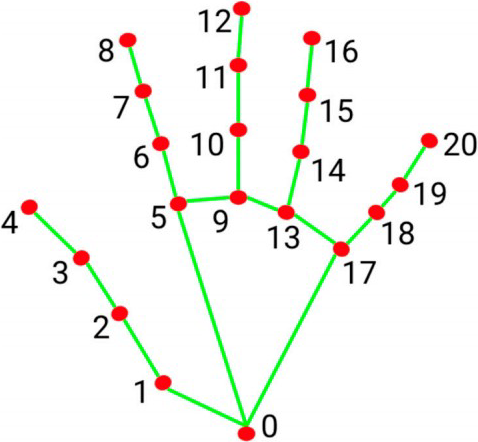
\includegraphics[width=\linewidth]{fig_skeleton}
\end{minipage}\hfill
\begin{minipage}[b]{0.44\columnwidth}
\centering
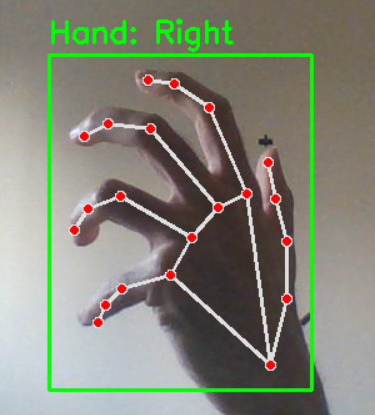
\includegraphics[width=\linewidth]{fig_overlay}
\end{minipage}
\caption{The 21-point hand skeleton \method{IGate} classifies (left) and the
runtime overlay the operator sees (right). The numbered joints are the indices
used throughout: 0 the wrist, 4 the thumb tip, 5 and 8 the index
metacarpophalangeal joint and tip that carry the rule's directional vector, and
20 the little-finger tip that separates LEFT from BACK
(Section~\ref{sec:packing}).}
\label{fig:skeleton}
\end{figure}

MediaPipe Hands produces 21 landmarks per detected hand
(Figure~\ref{fig:skeleton}), flattened to
\begin{equation}
\mathbf{f}_t=[x_1,y_1,z_1,\dots,x_{21},y_{21},z_{21}]^{\!\top}\in\mathbb{R}^{63}.
\label{eq:feat}
\end{equation}
Coordinates are normalised to the image frame, so the representation is
invariant to where the hand sits in view but \emph{not} to how large it appears;
Section~\ref{sec:gesture} finds that residual scale dependence to be the
strongest single predictor of cross-session transfer.

Landmark coordinates jitter frame to frame, so the geometric rule smooths its
input with a first-order exponential moving average,
\begin{equation}
\tilde{\mathbf{f}}_t=\alpha\,\mathbf{f}_t+(1-\alpha)\,\tilde{\mathbf{f}}_{t-1},
\qquad \alpha=0.35 ,
\label{eq:ema}
\end{equation}
and resets $\tilde{\mathbf{f}}$ whenever the hand is lost for longer than the
arbitration release time, so that a stale vector cannot carry across a gap. One
asymmetry follows from where \eqref{eq:ema} sits: it is applied inside the rule,
not in the shared perception path, so the learned classifier receives
$\mathbf{f}_t$ unsmoothed. Section~\ref{sec:inflight} states the consequence for
the comparison between them.

A detection is admitted only after it repeats, hands on two consecutive frames
and faces on one, since a spurious hand issues a command while a spurious face
only widens what is already permitted.

\subsection{Two Gesture Vocabularies}
\label{sec:vocab}

\method{IGate} carries two gesture classifiers, and they decode
\emph{different vocabularies}: the rule reads where the index finger points, the
classifier reads the configuration of the whole hand. A pose meaning FORWARD to
one is not a degraded FORWARD to the other but an input it has no reading for,
so every comparison in Section~\ref{sec:results} cues each arm on the vocabulary
it decodes, and Section~\ref{sec:opgesture} reports three figures rather than
two.

\textit{Geometric rule.} With $\mathbf{p}_{\mathrm{tip}}$ and
$\mathbf{p}_{\mathrm{mcp}}$ the index tip and metacarpophalangeal joint
(landmarks 8 and 5), the directional vector is
\begin{equation}
\mathbf{v}=\mathbf{p}_{\mathrm{tip}}-\mathbf{p}_{\mathrm{mcp}},
\label{eq:vindex}
\end{equation}
and a lateral or vertical component is emitted when the corresponding element of
$\mathbf{v}$ exceeds $\theta_{\mathrm{dir}}=0.10$ in normalised units. Depth is
inferred not from a pose but from a \emph{change}: with $A_t$ the landmark
bounding-box area,
\begin{equation}
\Delta s_t=\frac{A_t-A_{t-1}}{A_{t-1}},
\label{eq:deltas}
\end{equation}
and FORWARD or BACK is emitted when $|\Delta s_t|$ exceeds
$\theta_{\mathrm{scale}}=0.18$. Equation~\eqref{eq:deltas} is a difference
between consecutive frames and is not normalised by $\Delta t$, so the same
physical motion yields different values at different frame rates;
Section~\ref{sec:depth} measures what that costs. The rule emits compound
labels, so $\mathbf{v}$ and $\Delta s_t$ can both fire on one frame. A stability
gate suppresses a depth component until the whole label has repeated for two
frames, since a single noisy frame can assert \eqref{eq:deltas} but not sustain
it.

\textit{Learned classifier.} The 63-dimensional vector is standardised to zero
mean and unit variance and classified by a support vector machine with a radial
basis function kernel,
\begin{equation}
f(\mathbf{x})=\sum_{i}\alpha_i y_i\,
\exp\!\left(-\gamma\lVert\mathbf{x}_i-\mathbf{x}\rVert^2\right)+b ,
\label{eq:svm}
\end{equation}
with $C=10$ and $\gamma$ set by the scale heuristic, over the same seven classes,
fitted on a stratified 75/25 split at seed 42. The runtime takes the arg-max of
the calibrated class posteriors rather than the raw decision function.

The classifier is selected explicitly at launch, validated before the aircraft is
armed, and recorded in the run manifest with the model's SHA-256; a startup
self-test confirms that the branch which executes is the one requested, and a
released regression test fails on any run whose manifest and per-frame latency
columns disagree. The arbitration trials of Section~\ref{sec:results} were flown
with the rule arm. Sections~\ref{sec:opgesture} and~\ref{sec:inflight} report
both arms measured through the aircraft, on the ground and in flight.

\subsection{Face Following}
\label{sec:facefollow}

Face following aligns the operator with the image centre and holds a standoff.
With $(e_x,e_y)$ the pixel offset of the face box centre from the image centre
and $e_z=a^{\star}-\bar{a}_t$ the deviation of the smoothed box area fraction
$\bar{a}_t$ from its target $a^{\star}$, the controller is proportional with
deadbands and clipping,
\begin{equation}
u=\operatorname{clip}\!\big(k\,e\cdot\mathbb{1}[\,|e|>\delta\,],\;
u_{\min},u_{\max}\big),
\label{eq:follow}
\end{equation}
with $k_{\mathrm{yaw}}=0.20$, $k_{\mathrm{ud}}=0.12$ and
$k_{\mathrm{fb}}=0.30$ on $10^{3}e_z$; limits $\pm20$, $\pm40$ and $\pm40$;
deadbands $\delta=18$~px laterally and $0.008$ in area fraction. Smoothing is
applied to the \emph{measurement} rather than to the command, an area EMA at
$\alpha=0.25$, so that the deadband acts on a stable estimate. The loop is rate
limited to 15~Hz independently of the frame rate.

The target is $a^{\star}=0.075$ of frame area, which is a control quantity and
not a distance until something calibrates it. Section~\ref{sec:identity}
supplies that calibration from the envelope sweep and places $a^{\star}$ at a
standoff of 0.94~m.

\subsection{Session-Level Identity Gate}
\label{sec:gate}

At startup the operator enrols: $N=20$ accepted crops are embedded and averaged
into a template $E_{\mathrm{auth}}=\tfrac{1}{N}\sum_{i}\phi(c_i)$, replacing an
earlier single-crop enrolment that made the session template a hostage to one
frame. Each later crop $c_t$ yields the cosine similarity
$S_t=\langle \phi(c_t),E_{\mathrm{auth}}\rangle$. Authorization $a_t$ is a
Schmitt trigger rather than a per-frame comparison,
\begin{equation}
a_t=
\begin{cases}
1, & S_t\ge\tau_{\mathrm{on}},\\
0, & S_t<\tau_{\mathrm{off}} \text{ for } k \text{ consecutive frames},\\
a_{t-1}, & \text{otherwise},
\end{cases}
\label{eq:gate}
\end{equation}
with $\tau_{\mathrm{on}}=0.55$, $\tau_{\mathrm{off}}=0.45$ and $k=3$. The hold
branch distinguishes \eqref{eq:gate} from a bare threshold
(Section~\ref{sec:hysteresis}).

Detection and recognition are separate stages: detection must be cheap enough to
run on a large fraction of frames, while recognition must be accurate on a small
crop and is affordable only at a lower rate. MediaPipe supplies the box $b_t$,
whose padded crop is resized to $112\times112$ and embedded by $\phi(\cdot)$, a
MobileFaceNet~\cite{chen2018mobilefacenets} trained on WebFace600K under the
ArcFace additive angular margin loss~\cite{deng2019} and exported to ONNX. The
embedding is therefore used outside the pipeline it was trained in, which aligns
each crop onto five facial landmarks and pairs the network with a
RetinaFace~\cite{deng2020retinaface} detector;
Section~\ref{sec:identity} treats that as one untested candidate for the
operational false rejection rate.

Separating the stages separates their time constants, and the two are not
interchangeable. Arbitration holds its face predicate across detection gaps for
2.0~s so mode selection does not flicker on a low-frame-rate stream; identity
accepts a crop only if its detection is younger than $\Delta_{\max}=0.35$~s,
because re-embedding a stale box feeds the network whatever now occupies a
region the face has left. Section~\ref{sec:staleness} reports what happened when
both read one predicate.

\textit{What the gate does not establish.} A gesture is admitted when a hand is
present and $a_t=1$. These are two independent tests over the frame, not an
association: the deployed perception path returns a single hand and never binds
it to the authorized face. Any hand in view therefore commands the aircraft
while the enrolled operator is also in view. The gate establishes operator
presence, not command provenance, and Section~\ref{sec:limitations} treats
closing that gap as the most valuable extension.

With the gate disabled, target selection falls back to the largest face box by
area and the single hand the detector returns; Section~\ref{sec:hysteresis}
measures that configuration as an ablation.

\subsection{Deterministic Arbitration}
\label{sec:arb}

\begin{figure}[t]
\centering
\resizebox{0.95\columnwidth}{!}{% Generated by tello_gesture_py/src/gestures/build_design_figures.py
% Do not edit: every value here is read from the deployed configuration.

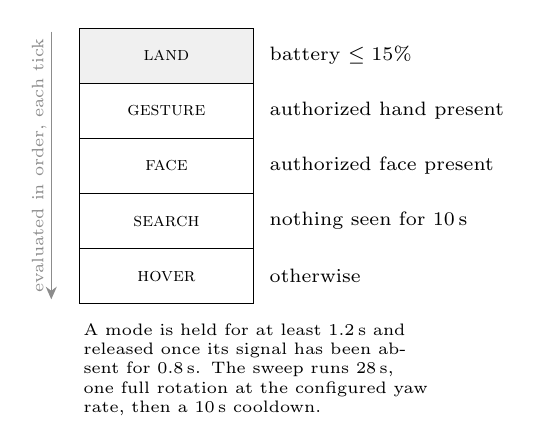
\begin{tikzpicture}[x=1mm,y=1mm]

\tikzset{
  blk/.style   = {draw, line width=0.4pt, inner sep=3pt, align=center,
                  minimum height=6.5mm, font=\scriptsize},
  wide/.style  = {blk, text width=20mm},
  narrow/.style= {blk, text width=17mm},
  gate/.style  = {wide, fill=black!4},
  aux/.style   = {wide, draw=black!35, text=black!55},
  flow/.style  = {-{Stealth[length=1.6mm,width=1.4mm]}, line width=0.4pt},
  aside/.style = {flow, densely dashed, draw=black!55},
  lbl/.style   = {font=\fontsize{6}{7}\selectfont, inner sep=1.5pt},
  grp/.style   = {draw=black!25, line width=0.3pt, rounded corners=1pt,
                  inner sep=0pt},
}


\node[blk, text width=20mm, minimum height=7.0mm, anchor=north west, fill=black!6] (m0) at (0,3.5) {\textsc{land}};
\node[font=\scriptsize, anchor=west] at (23,0.0) {battery $\le 15\%$};
\node[blk, text width=20mm, minimum height=7.0mm, anchor=north west, fill=white] (m1) at (0,-3.5) {\textsc{gesture}};
\node[font=\scriptsize, anchor=west] at (23,-7.0) {authorized hand present};
\node[blk, text width=20mm, minimum height=7.0mm, anchor=north west, fill=white] (m2) at (0,-10.5) {\textsc{face}};
\node[font=\scriptsize, anchor=west] at (23,-14.0) {authorized face present};
\node[blk, text width=20mm, minimum height=7.0mm, anchor=north west, fill=white] (m3) at (0,-17.5) {\textsc{search}};
\node[font=\scriptsize, anchor=west] at (23,-21.0) {nothing seen for 10\,s};
\node[blk, text width=20mm, minimum height=7.0mm, anchor=north west, fill=white] (m4) at (0,-24.5) {\textsc{hover}};
\node[font=\scriptsize, anchor=west] at (23,-28.0) {otherwise};
\draw[flow, draw=black!45] (-3.5,3.0) -- (-3.5,-31.0) node[lbl, midway, rotate=90, anchor=south, text=black!45] {evaluated in order, each tick};
\node[lbl, text width=44mm, anchor=north west, align=left] at (0,-33.5) {A mode is held for at least 1.2\,s and released once its signal has been absent for 0.8\,s. The sweep runs 28\,s, one full rotation at the configured yaw rate, then a 10\,s cooldown.};
\end{tikzpicture}
}
\caption{Arbitration. The condition list is evaluated in order on every control
tick and the first match selects the mode.}
\label{fig:hfsm}
\end{figure}

A hierarchical state machine selects one mode $m_t$ per control tick by the
first satisfied condition in a fixed priority order (Figure~\ref{fig:hfsm}), so
that a low-battery condition preempts everything and an authorized gesture
preempts face following. The hold and release times exist so that intermittent
detection does not translate into mode chatter.

The sweep runs 28~s, one full rotation at the deployed yaw rate of
approximately 13\textdegree/s. Section~\ref{sec:flightbehaviour} reports the
measurement that set that duration and why the yaw rate is not raised instead.

\subsection{Reason-Only Language Model}
\label{sec:reasondesign}

An early design placed a language model in the control loop, mapping perception
summaries to commands. Three properties ruled it out: its inference latency is
of the same order as the interval between commands; its outputs are not
deterministic, which removes the property that makes a failure reconstructible
from a log; and under ambiguous perception it was the states where a command
matters most that produced the least defensible suggestions.

\method{IGate} therefore confines the model to explanation. Every command is
computed by \eqref{eq:gate} and the state machine, and a structured summary of
each decision then goes to a local Qwen2.5-0.5B instance, which returns one
sentence for the log. Its latency and its errors are observable without being
consequential, which makes Section~\ref{sec:llm} a measurement of the design
decision rather than of a component in service.

Table~\ref{tab:design} lists every parameter set above that
Section~\ref{sec:results} measures, with the figure each one returned. Its left
half is read from the deployed configuration by the table's own generator, so
the specification in this section and the artefact that flew cannot drift
apart.

\begin{table*}[t]
\caption{Parameters Section~\ref{sec:system} specifies and Section~\ref{sec:results} measures. The left half is generated from the deployed configuration.}
\label{tab:design}
\centering
\footnotesize
\setlength{\tabcolsep}{5pt}
\renewcommand{\arraystretch}{1.05}
\begin{tabular}{@{}llccl@{}}
\toprule
Parameter & Deployed value & Set in & Measured in & Result \\
\midrule
Hand, face throttle & 2, 4 frames & \S\,\ref{sec:perception} & \S\,\ref{sec:runtime} & duty 50\%, 25\%; 22.3~fps \\
EMA $\alpha$ (rule only) & 0.35 & \S\,\ref{sec:perception} & \S\,\ref{sec:inflight} & arms not input-matched \\
$\theta_{\mathrm{dir}}$ & 0.1 & \S\,\ref{sec:vocab} & \S\,\ref{sec:opgesture} & lateral $F_1$ 0.921 / 0.937 / 0.855 \\
$\theta_{\mathrm{scale}}$ on $\Delta s_t$ & 0.18 & \S\,\ref{sec:vocab} & \S\,\ref{sec:depth} & depth $F_1$ 0.008 / 0.066; pose form 0.447 / 0.567 \\
Depth stability streak & 2 frames & \S\,\ref{sec:vocab} & \S\,\ref{sec:depth} & gated vs ungated differ by 0.004 \\
Face-follow target $\rho^{\star}$ & 0.075 of frame & \S\,\ref{sec:facefollow} & \S\,\ref{sec:identity} & 0.94~m, band 0.90--1.00~m \\
$\tau_{\mathrm{on}}$ & 0.55 & \S\,\ref{sec:gate} & \S\,\ref{sec:identity} & FRR 19.3\% in flight; 35.1\% ungated at the same threshold \\
$\tau_{\mathrm{off}}$, $k$ & 0.45, 3 & \S\,\ref{sec:gate} & \S\,\ref{sec:hysteresis} & 15.7 vs 78.5 mode switches/min; impostor 0.0\% $\to$ 5.6\% \\
Enrolment $N$ & 20 crops & \S\,\ref{sec:gate} & \S\,\ref{sec:identity} & genuine cluster $0.770\pm0.109$ \\
$\Delta_{\max}$ crop freshness & 0.35~s & \S\,\ref{sec:gate} & \S\,\ref{sec:staleness} & background share 56\% $\to$ 20\%; authorized 41\% $\to$ 68\% \\
Arbitration face hold & 2.0~s & \S\,\ref{sec:gate} & \S\,\ref{sec:staleness} & search decisions 130 $\to$ 4 \\
Mode hold, release & 1.2~s, 0.8~s & \S\,\ref{sec:arb} & \S\,\ref{sec:results} & 149/149 trials produced the specified behaviour \\
Search sweep & 28~s & \S\,\ref{sec:arb} & \S\,\ref{sec:flightbehaviour} & 318\textdegree{} over 22 episodes; 60\textdegree{} at the 5~s originally specified \\
Battery failsafe & 15\% & \S\,\ref{sec:arb} & \S\,\ref{sec:flightbehaviour} & 11 consecutive landings, 91\% $\to$ 21\% \\
LLM decision rate & 1~Hz, no actuation & \S\,\ref{sec:reasondesign} & \S\,\ref{sec:llm} & 1766~ms mean, 5.5\% timeouts \\
\bottomrule
\end{tabular}
\end{table*}


\section{Experiments}
\label{sec:setup}

\subsection{Instrumentation and Protocol}

Each launch writes a timestamped run directory containing telemetry, decision,
per-frame performance and trial logs, with a manifest recording configuration,
git commit, library versions and host. All tables here are generated from those
logs by a released script.

Two conventions make the latency figures meaningful. A throttled stage
contributes a sample only on frames where it executed, since averaging executed
and skipped frames yields a figure describing neither; and frames are deduplicated
by sequence number before any rate is computed, as the control loop can iterate
faster than the decoder delivers.

\subsection{Gesture Datasets}

Four sessions of seven gesture classes (CENTER, LEFT, RIGHT, UP, DOWN, FORWARD,
BACK) were captured at 400 images per class under deliberately different
conditions rather than as replicates, so that transfer could be attributed to a
stated variable. Session A is the reference condition, a laboratory in daylight
against a uniform blue wall separating hand from background in intensity and hue.
Sessions B and C were recorded seven months later in two domestic rooms at night
under artificial light, chosen to degrade that separability: B's background is
close to skin tone, removing the chroma cue, and C uses a mixed domestic
background. Those three vary illumination and background together, so neither can
be attributed alone. Session D closes that cell: a domestic room with a cluttered
backdrop, recorded in daylight, holding the illumination of A while taking the
background of B and C.

The conditions differ in chroma rather than in brightness. Mean grey level is
almost constant across the four sessions, at 114, 118, 116, 123, but the blue-minus-red channel
separation is 74 in A against 2, 0, -27 in B, C and D: only the reference condition
offers a hue cue separating hand from backdrop, and it offers no more light than
the others. Landmark extraction yielded 2715, 2345, 2613, 2784 usable samples of 2800. The shortfall in
B concentrates in UP and DOWN, where the hand approached the frame edge, and is
itself a measurement of the condition.

\subsection{Trial Protocol and Validity Rule}

Eight scenarios were defined. Five require flight; three concern mode arbitration
only and were additionally run on a webcam harness executing the identical
perception, gating and arbitration code, which compares both identity-gate
configurations without consuming flight time. The operator opens a trial with a
key press, performs the behaviour and resolves it as pass or fail. Trial counts
differ by scenario because their costs differ: search and reacquisition chain
within one flight, whereas each failsafe trial needs a separate takeoff.

A flight trial counts only if the aircraft was airborne within the trial window,
verified from the command log; the rule is uniform and does not select on
outcome. Of 150 flight trials, one was excluded, having been opened after a
failsafe landing and before the next takeoff.

% =====================================================================
\section{Results}
\label{sec:results}

\subsection{Scenario Validation}

Eight scenarios test whether the arbitration layer of
Section~\ref{sec:arb} produces its specified behaviour. All 149 valid in-flight
trials did: authorized gesture accepted (24), face following activates (31),
search starts after loss (48), target reacquired (33), battery failsafe landing
(13). The three arbitration scenarios were additionally run on the webcam
harness under both identity-gate configurations, where 61 of 61 trials passed in
the deployed configuration and one of 60 failed under the bare-threshold
ablation --- the direct evidence for the Schmitt trigger, analysed in
Section~\ref{sec:hysteresis}. The Wilson interval is the one to quote when every
trial passes, since the normal approximation collapses to zero width at $p=1$;
at $n=24$ it is [86, 100]\%.

A ceiling establishes that the arbitration layer behaves as designed and nothing
more: with no trial failing it cannot discriminate between correct and incorrect
perception beneath it. The experiments that follow address those layers
directly.

\subsection{Runtime Performance}
\label{sec:runtime}

\begin{table}[t]
\caption{Runtime performance in flight. Latency is conditioned on frames where the stage actually ran; the duty cycle reports how often that was.}
\label{tab:runtime}
\centering
\footnotesize
\setlength{\tabcolsep}{4pt}
\renewcommand{\arraystretch}{1.02}
\begin{tabular}{@{}lrrrr@{}}
\toprule
Stage & Mean & Median & p95 & Duty \\
& (ms) & (ms) & (ms) & (\%) \\
\midrule
Hand detection (MediaPipe Hands) & 26.69 & 25.17 & 36.90 & 50 \\
Face detection (MediaPipe) & 7.14 & 6.97 & 9.47 & 25 \\
Face embedding + cosine match & 13.01 & 13.38 & 16.63 & 25 \\
Mode-manager update & 0.02 & 0.02 & 0.04 & 100 \\
Command execution & 0.61 & 0.01 & 2.86 & 100 \\
Frame age (decode + queue) & 9.05 & 3.99 & 30.52 & 100 \\
End-to-end camera-to-command & 19.08 & 18.62 & 55.16 & 100 \\
\midrule
Video stream & \multicolumn{4}{r}{22.3 fps} \\
\bottomrule
\end{tabular}
\end{table}


Table~\ref{tab:runtime} reports latency over 557~s airborne and 12{,}419 frames.
Median end-to-end camera-to-command latency is 18.6~ms (p95 55.2~ms) at 22.3~fps.
Frame age at consumption, the decode and queue delay a host-side measurement
omits, contributes a median 4.0~ms and p95 30.5~ms.

Stage costs are higher in flight than on the ground, hand detection rising from
24.4 to 26.7~ms and face embedding from 9.0 to 13.0~ms, consistent with motion
blur and vibration increasing detector workload. Table~\ref{tab:runtime} is
built from the longest airborne run, which predates the classifier-latency
column; measured over the hover-locked captures of
Section~\ref{sec:inflight}, gesture inference costs a mean 0.84~ms for the SVM
and 0.07~ms for the rule against 26.7~ms for hand detection, so the accuracy
difference between the two arms is bought for under a millisecond and the choice
is not a latency trade-off.

\subsection{Cross-Session Gesture Classification}
\label{sec:gesture}

\begin{table}[t]
\caption{Transfer accuracy $\uparrow$, training on the row session and testing on the column. A daylight/uniform, B and C artificial/non-uniform, D daylight/non-uniform.}
\label{tab:transfer}
\centering
\footnotesize
\setlength{\tabcolsep}{4pt}
\renewcommand{\arraystretch}{1.02}
\begin{tabular}{@{}llrrrr@{}}
\toprule
\multicolumn{2}{@{}l}{Train} & \multicolumn{4}{c}{Test} \\
\cmidrule(l){3-6}
 & & A & B & C & D \\
\midrule
A & \footnotesize day/unif. & -- & 0.815 & 0.842 & 0.930 \\
B & \footnotesize art./clutter & 0.709 & -- & 0.969 & 0.977 \\
C & \footnotesize art./clutter & 0.471 & 0.509 & -- & 0.842 \\
D & \footnotesize day/clutter & 0.638 & 0.737 & 0.966 & -- \\
\bottomrule
\end{tabular}
\end{table}





\begin{figure}[t]
\centering
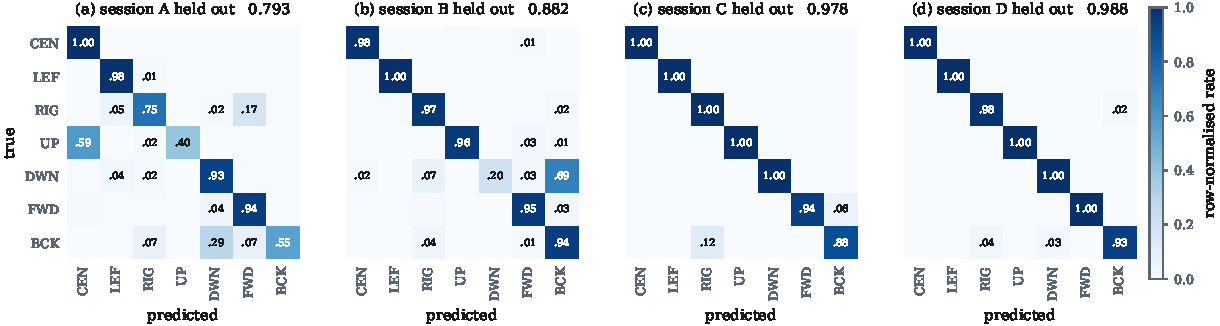
\includegraphics[width=0.92\columnwidth]{fig_sessions}
\caption{Row-normalised confusion, each session held out and predicted by a
classifier trained on the other three.}
\label{fig:sessions}
\end{figure}

The classifier evaluated in this section is the RBF-SVM. The protocol result
below is a statement about evaluation methodology and holds for any classifier
scored this way. Evaluated within each session under a stratified random split,
the SVM reaches 0.997, 0.988, 1.000 and 1.000 on sessions A, B, C and D. The
protocol does not separate the reference condition from the three degraded ones:
it returns 1.000 on both C and D and its lowest figure, 0.997, on A, the
condition in which hand and background are most separable. A protocol that ranks
the hardest capture conditions above the easiest is characterising the recording
rather than the classifier, and each session added has made that clearer rather
than diluting it.

The mechanism is visible in the sampling density: within session A accuracy
rises monotonically with the frames retained per class, 0.9486 at 100, 0.9840 at
250, 0.9971 at 400. Frames captured milliseconds apart during a continuous
recording of a static pose are near-identical in landmark space, so a random
split distributes near-duplicates across both partitions and accuracy rises with
sampling density instead of saturating. That is the signature of leakage, and is
consistent with the subject-independence analysis of Varga~\cite{varga2026}.

Leave-one-session-out evaluation gives 0.793, 0.882, 0.978 and 0.988
(Figure~\ref{fig:sessions}), a mean of 0.910. Over A--C alone the mean is 0.872,
and adding D raises the A fold from 0.756 to 0.793.

Table~\ref{tab:transfer} reports the full matrix, and transfer is markedly
asymmetric: A reaches 0.815, 0.842 and 0.930 on B, C and D as a training set,
whereas C reaches only 0.471 and 0.509 on A and B while reaching 0.842 on D,
with which it shares a cluttered backdrop. A clean backdrop is therefore the
more valuable training condition and the more misleading test condition.
Elapsed time is not the binding variable, since B, C and D were recorded on the
same day and span the full range of the matrix.

Three sessions cannot say which condition is responsible: A is daylight against
a uniform wall while B and C are artificial light against cluttered rooms, so
the two factors move together. Session D, daylight against a cluttered room, was
captured to separate them, and does not. Grouping the twelve ordered pairs by
what changes gives 0.739 where neither factor moves (2 pairs), 0.784 for
background alone (2), 0.880 for illumination alone (4) and 0.709 where both move
(4). The two single-factor groups order as expected but their ranges overlap
almost completely, 0.638--0.930 against 0.737--0.977, and the difference is not
significant ($p=0.53$); at two against four the smallest attainable $p$ is
0.067, so the design cannot reach significance even in principle.

A post-hoc analysis of the released features suggests the axis it misses. Median
hand scale in landmark space differs by a factor of 3.5 across the four
sessions, and the fraction of a test session's scale distribution lying inside
the training session's 5th--95th percentile range correlates with transfer at
$r=0.76$ over the 12 ordered pairs, against 0.30 for shared background and
$-0.09$ for shared illumination. Being directional, it also accounts for the
asymmetry the two-factor model cannot: C$\rightarrow$A pairs the lowest coverage
with the lowest accuracy and D$\rightarrow$C the highest with the highest. It is
exploratory --- chosen after seeing the matrix, $n=12$, and partly definitional,
since coverage of a test distribution by a training one restates covariate shift
rather than explaining it --- and is a caveat on the grouping rather than a
replacement for it.

The dominant error differs by fold. With session A held out, 59\% of UP samples
are assigned to CENTER and UP recovers only $F_1=0.57$. With session B held out,
69\% of DOWN samples are assigned to BACK, and DOWN falls to $F_1=0.33$. FORWARD
and BACK are separated by apparent hand size rather than by finger direction,
and BACK accordingly acts as an attractor for samples whose scale is
uninformative. Standoff was varied during capture but was neither held to a
common range nor recorded per frame, so the two scale-derived classes meet test
distributions their training set never covered. With C and D held out, accuracy
reaches 0.978 and 0.988 and no off-diagonal cell exceeds 0.12.
Section~\ref{sec:depth} reports an independent measurement of the same
scale-cue sensitivity in flight.

\subsection{Gesture Classification Through the Aircraft}
\label{sec:opgesture}

Both protocols above score the classifier on frames a webcam captured. A third measurement scores it on frames the aircraft encoded,
transmitted and the host decoded. With the drone powered and streaming on the
ground and its propellers removed, a cued protocol named one of the seven classes,
allowed 5~s to form it and recorded 6~s, over 42 holds in six rounds of
randomised class order. What the measurement needs from the aircraft is its
codec, its optics and its link, none of which require flight.

The SVM reaches 0.783 over all 2947 cued frames, and 0.809 over the 42 holds,
the hold being the independent unit because the operator was cued once and
formed the gesture once. A hand was detected in every frame, so the loss is
entirely misclassification and none of it is hidden in frames that issued no
command. The frame-level interval is the narrower of the two and the optimistic
one: frames within a hold are the same pose milliseconds apart, so treating them
as independent repeats in miniature the error this section identifies in
within-session splitting.

The three protocols therefore give 0.997, 0.910 and 0.783 on the RBF-SVM, each
stricter than the last.

The rule scores 0.287 on those same frames, and that figure is not its accuracy
in service: the lateral component of $\mathbf{v}$ exceeds $\theta_{\mathrm{dir}}$
in under 3\% of frames of every class, so these poses do not encode pointing and
the rule cannot emit LEFT or RIGHT from them at all
(Section~\ref{sec:vocab}).

The deployed path was therefore captured on the vocabulary it does decode, under
the same protocol and through the same pipeline, with the depth-stability gate
applied so that the figure is the command the aircraft would issue rather than
the classifier's raw output. Over 2625 cued frames in 36 holds it reaches 0.584
[0.565, 0.603] and 0.611 per hold, at a detection rate of 0.890. A further six holds are excluded, in which
the lateral commands are inverted without exception, 211 of 211 frames cued LEFT
read RIGHT and 216 of 216 cued RIGHT read LEFT. A total inversion means the cue
and the decoder disagreed on which frame the word names rather than that either
performed poorly. The holds are excluded rather than relabelled, since
recovering a cue from the classifier's own output would be circular.

That aggregate conceals a split. On the four directional commands the rule was
built for it reaches $F_1$ of 0.921, 0.937, 0.635 and 0.855; on the two depth
commands it reaches 0.008 and 0.066. The deployed system is a competent
four-direction pointer with a depth channel that barely functions, which is
visible in the flight logs, where FORWARD and BACK together account for 47 of the
980 gesture components emitted.

In the SVM's static-pose capture only two off-diagonal cells exceed 0.10, and
both collapse into BACK: 0.72 of frames cued RIGHT and 0.71 cued FORWARD --- the
classes separated by the smallest geometric margin and by apparent scale, and
the same two the held-out folds identify, reached independently through
different optics. The rule's failures fall on the depth classes alone, which is
what a different vocabulary predicts.

\subsection{Both Classifiers in Flight}
\label{sec:inflight}

\begin{table}[t]
\caption{Gesture classification in flight $\uparrow$, hover-locked cued capture. Recall is unconditioned; the bracketed figure conditions on detection. Per-hold scores each of the 42 holds by majority vote.}
\label{tab:inflight}
\centering
\footnotesize
\setlength{\tabcolsep}{3pt}
\renewcommand{\arraystretch}{1.02}
\begin{tabular}{@{}lrrrrrr@{}}
\toprule
& \multicolumn{3}{c}{RBF-SVM} & \multicolumn{3}{c}{Rule} \\
\cmidrule(lr){2-4}\cmidrule(lr){5-7}
Class & Recall & Prec. & $F_1$ & Recall & Prec. & $F_1$ \\
\midrule
CENTER & 0.988 & 0.941 & 0.964 & 0.881 & 0.567 & 0.690 \\
LEFT & 0.980 & 0.736 & 0.841 & 0.999 & 1.000 & 0.999 \\
RIGHT & 0.985 & 0.685 & 0.808 & 0.968 & 0.997 & 0.982 \\
UP & 0.999 & 1.000 & 0.999 & 0.854 & 0.548 & 0.668 \\
DOWN & 0.920 & 1.000 & 0.958 & 0.908 & 1.000 & 0.952 \\
FORWARD & 0.777 (0.858) & 1.000 & 0.874 & 0.000 & 0.000 & 0.000 \\
BACK & 0.336 & 0.859 & 0.483 & 0.008 & 0.750 & 0.017 \\
\midrule
Per frame & \multicolumn{3}{c}{0.850 [0.840, 0.860]} & \multicolumn{3}{c}{0.651 [0.638, 0.664]} \\
Per hold & \multicolumn{3}{c}{0.905 [0.779, 0.962]} & \multicolumn{3}{c}{0.714 [0.564, 0.828]} \\
Detection & \multicolumn{3}{c}{0.986} & \multicolumn{3}{c}{0.984} \\
\bottomrule
\end{tabular}
\end{table}


The measurements above are taken on the ground. A final protocol puts both
classifiers in the air under the identical cue. Cued holds are not flyable in a
domestic room with actuation live, since a sustained directional command
translates roughly 3.9~m in six seconds, so the captures use a hover lock:
perception, gating, arbitration, the depth stability gate and the command
computation run and are logged exactly as deployed, while the transmitted
radio-control command is held at zero. Suppression is applied at the transmit
boundary, so nothing upstream branches on it and the logged command is the one
the aircraft would have received.

Each arm was cued on the vocabulary it decodes over 42 holds in six rounds of
randomised class order, at a matched standoff inside the authorization envelope
of Section~\ref{sec:identity}: median 0.85~m for the SVM arm and 0.89 and
0.81~m for the two rule captures. These 84 holds are a separate protocol and are
not among the 270 trials. Table~\ref{tab:inflight} reports the result. The SVM
reaches 0.850 per frame [0.840, 0.860] and 0.905 per hold, the rule 0.651 and
0.714, with hand detection above 0.98 in both.

One asymmetry bounds the comparison: \eqref{eq:ema} is applied inside the rule
rather than in the shared perception path, so the rule is scored on smoothed
landmarks and the SVM on raw ones. The arms are compared as deployed
capabilities, not as classifiers on matched input; the smoothing favours the
rule, so it cannot account for the direction of the gap.

The gesture classifier does not degrade in flight as the identity gate does. It
reaches 0.783 on the ground and 0.850 airborne through the aircraft's optics,
against 0.910 held out across sessions and 0.997 within session: what governs
the gesture figure is the evaluation protocol, not the platform. The ground
capture did not record apparent face size, so the comparison between 0.783 and
0.850 cannot be conditioned on framing, and the supported claim is the weaker
one --- flight produced nothing resembling the order-of-magnitude collapse the
identity gate shows.

The comparison was specified before it was flown. A preregistration fixed the
primary metric as per-hold accuracy on the depth channel, each arm on its own
vocabulary; the sample size at 42 holds per arm, with the all-class comparison
declared underpowered and descriptive; the frozen model and its SHA-256; and an
exclusion rule admitting only declared operator error, excluded and never
relabelled. It recorded one directional prediction, that the SVM's RIGHT would
collapse into BACK as it had on the ground, at $F_1$ 0.433 against the rule's
0.937. \emph{That prediction was disconfirmed.} In flight the SVM reads RIGHT
correctly on 0.985 of cued frames and BACK never; the confusion reversed
direction, BACK becoming the error source rather than its target and dividing
between LEFT at 0.33 and RIGHT at 0.30. The document is released with the code.
Two caveats on its status: it was written to disk before the first flight but was
not placed under version control, so its date rests on a file timestamp, and it
specifies a cued protocol whose actuation assumption was revised to the hover
lock described above.

No static class falls below 0.92 recall on the SVM, DOWN reaching that figure
exactly; on $F_1$ two fall short, LEFT at 0.841 and RIGHT at 0.808, because
BACK leaks into both and recall does not show it. Two of five reach 0.92 on the
rule, CENTER, UP and DOWN falling short at 0.881, 0.854 and 0.908. The two
classifiers separate mainly on the depth channel, as Section~\ref{sec:depth}
predicts: of the 0.199 gap in per-frame accuracy, 0.162 -- 82\% -- is
contributed by FORWARD and BACK alone. The remaining 0.037 falls on UP and
CENTER, the two static classes the rule reads worst; their relative shares are
sensitive to the small difference in frame counts between the two captures and
are not separated here.

\subsection{Depth Commands: Motion Cue versus Static Pose}
\label{sec:depth}

This experiment quantifies command contamination from the depth gesture
rule.

FORWARD and BACK are inferred from the relative change in hand bounding-box area
between consecutive frames, $\Delta s_t=(A_t-A_{t-1})/A_{t-1}$, compared against
a fixed threshold. The expression is not normalised by $\Delta t$, so at a
variable frame rate the same physical motion produces different values.

The in-flight capture of Section~\ref{sec:inflight} settles the design
question the defect raises. Expressed as a static pose and read by the SVM, the
same two commands reach 0.777 and 0.336 in flight against 0.000 and 0.008 for
the motion cue, measured on the same aircraft at the same standoff under the
same protocol. The pose formulation removes the motion cue's pathology outright:
FORWARD goes from unusable to 0.777, and none of the four failure modes set out
below applies to a configuration. BACK does not follow it, and its 0.336 is not a
residue of the motion problem but a second and independent one, diagnosed in
Section~\ref{sec:packing}. The hover-locked capture also rules out a
flight-specific suspicion: since the cue reads apparent hand size, the
aircraft's own motion might have triggered it, but over the lateral-cued frames
of the rule arm $|\Delta s_t|$ exceeded its threshold in 0.00\% of frames, the
figure the static-camera ground capture also returns. Telemetry puts the
aircraft at a median ground velocity of zero in all three axes throughout, so
this bounds \emph{hover drift} and not translation under an active command,
which remains unmeasured.

The missing normalisation is the lesser problem. A motion cue has no steady
state: the correct component fired in every one of the twelve depth holds but
occupied 9\% of the window, so for most of the time the operator was gesturing
the aircraft was told nothing, and the return stroke supplies the opposite
command unless made slower than the threshold --- 67\% of BACK holds emitted a
spurious FORWARD. It also costs detection, MediaPipe finding the hand in 0.70 of
depth-cued frames against 1.00 for every static class. The same two classes as
static poses reach $F_1$ of 0.447 and 0.567 against 0.008 and 0.066 on the same
camera. The $\Delta t$ defect is thus a consequence of choosing a motion cue
rather than an independent fault. The stability gate is close to inert against
it: gated and ungated accuracy differ by 0.004, the cue being too sparse for a
streak requirement to act on.

Across the 64 active gesture frames in the 22 trials where the operator issued
no depth gesture, 4 (6.2\%) carried a FORWARD or BACK component alongside the
commanded axis, and the aircraft received an uncommanded depth velocity. All 22
were scored as passes, correctly, since the aircraft moved in the commanded
direction, and the contamination appears only in the log -- corroborating
Section~\ref{sec:gesture}, where the same two classes transfer least well.

\subsection{Vocabulary Packing and Landmark Precision}
\label{sec:packing}

The SVM's one weak static class has a mechanism, and it is not the classifier.
Three of the seven trained poses share a closed fist and are distinguished by a
single extended digit: LEFT by the little finger, RIGHT by the thumb, BACK by
neither. Separating the in-flight frames cued BACK by what the classifier emitted shows
the distinguishing digit doing the separating. Little finger extension,
normalised by palm length, is 0.884 on the frames read as LEFT
against 0.551 on those read correctly, a difference of 0.333; the frames read as
RIGHT carry a thumb extension of 0.205 against 0.526. By majority vote the six
holds divide two to BACK, two to RIGHT and two to LEFT, so per-hold accuracy is
0.333 against 0.336 per frame: the one class here in which the two units agree,
because its errors are not brief excursions.

The two comparisons rest on different structure. The LEFT confusion is entirely
between holds -- two holds returned LEFT on every frame and no frame of the
other four was read LEFT -- so that contrast has two holds behind it and no
significance test is reported. The thumb contrast is within holds, the remaining
four each mixing BACK and RIGHT frames, and is the better supported of the two.
The effect size carries the argument: genuine LEFT poses measure 0.821, so on
the misread holds the estimator reported a little finger \emph{more} extended
than on the class it belongs to. The classifier is faithfully labelling the hand
it was given.

The direction of the confusion is itself informative. A pose family separated by
a single digit should confuse in whichever direction estimator error happens to
fall, not in a stable one, and the reversal between the ground capture, where
RIGHT collapsed into BACK, and flight, where BACK divides between LEFT and
RIGHT, is what that predicts. A classifier deficiency would be expected to
reproduce its direction.

The failure is therefore one of landmark estimation, not of classification, and
it follows from a vocabulary whose classes are separated by less than the
estimator resolves. A gesture set for a landmark-based recogniser should be
designed with a margin the estimator can hold, and single-digit distinctions on
an otherwise identical hand do not meet that condition.

The errors are also structured rather than uniform. Across the in-flight holds,
82\% of error episodes last ten frames or fewer, a median of five frames or
0.17~s, which at the deployed command rate displaces the aircraft by about
0.11~m and is invisible to an operator. The remaining 18\% run to eleven frames
or more, up to a sustained 5.98~s. At the deployed command rate that projects to
3.9~m of travel on a single uncorrected command; the figure is a projection,
since actuation was suppressed during the capture and the aircraft did not move.
Six of those ten episodes fall on BACK. An
operator judging the system by whether it behaves sees the first mode; only
per-frame logging distinguishes it from the second.

\subsection{Identity Verification: Offline and Operational}
\label{sec:identity}

\begin{table}[t]
\caption{False rejection of the enrolled operator $\downarrow$, in per cent, at the offline equal-error threshold and at the deployed one.}
\label{tab:frr}
\centering
\footnotesize
\setlength{\tabcolsep}{4pt}
\renewcommand{\arraystretch}{1.02}
\begin{tabular}{@{}lrr@{}}
\toprule
Condition & Frames & FRR (\%) \\
\midrule
Offline still images, $\tau=0.18$ & 13{,}410 & 0.32 \\
Drone in flight, $\tau=0.18$ & 684 & 7.3 \\
Drone in flight, $\tau=0.55$, per frame & 684 & 35.1 \\
Drone in flight, $\tau=0.55$, deployed gate & 684 & 19.3 \\
Drone on ground, $\tau=0.55$, per frame & 2792 & 16.7 \\
Drone on ground, $\tau=0.55$, deployed gate & 2792 & 9.2 \\
\bottomrule
\end{tabular}
\end{table}


\begin{figure*}[t]
\centering
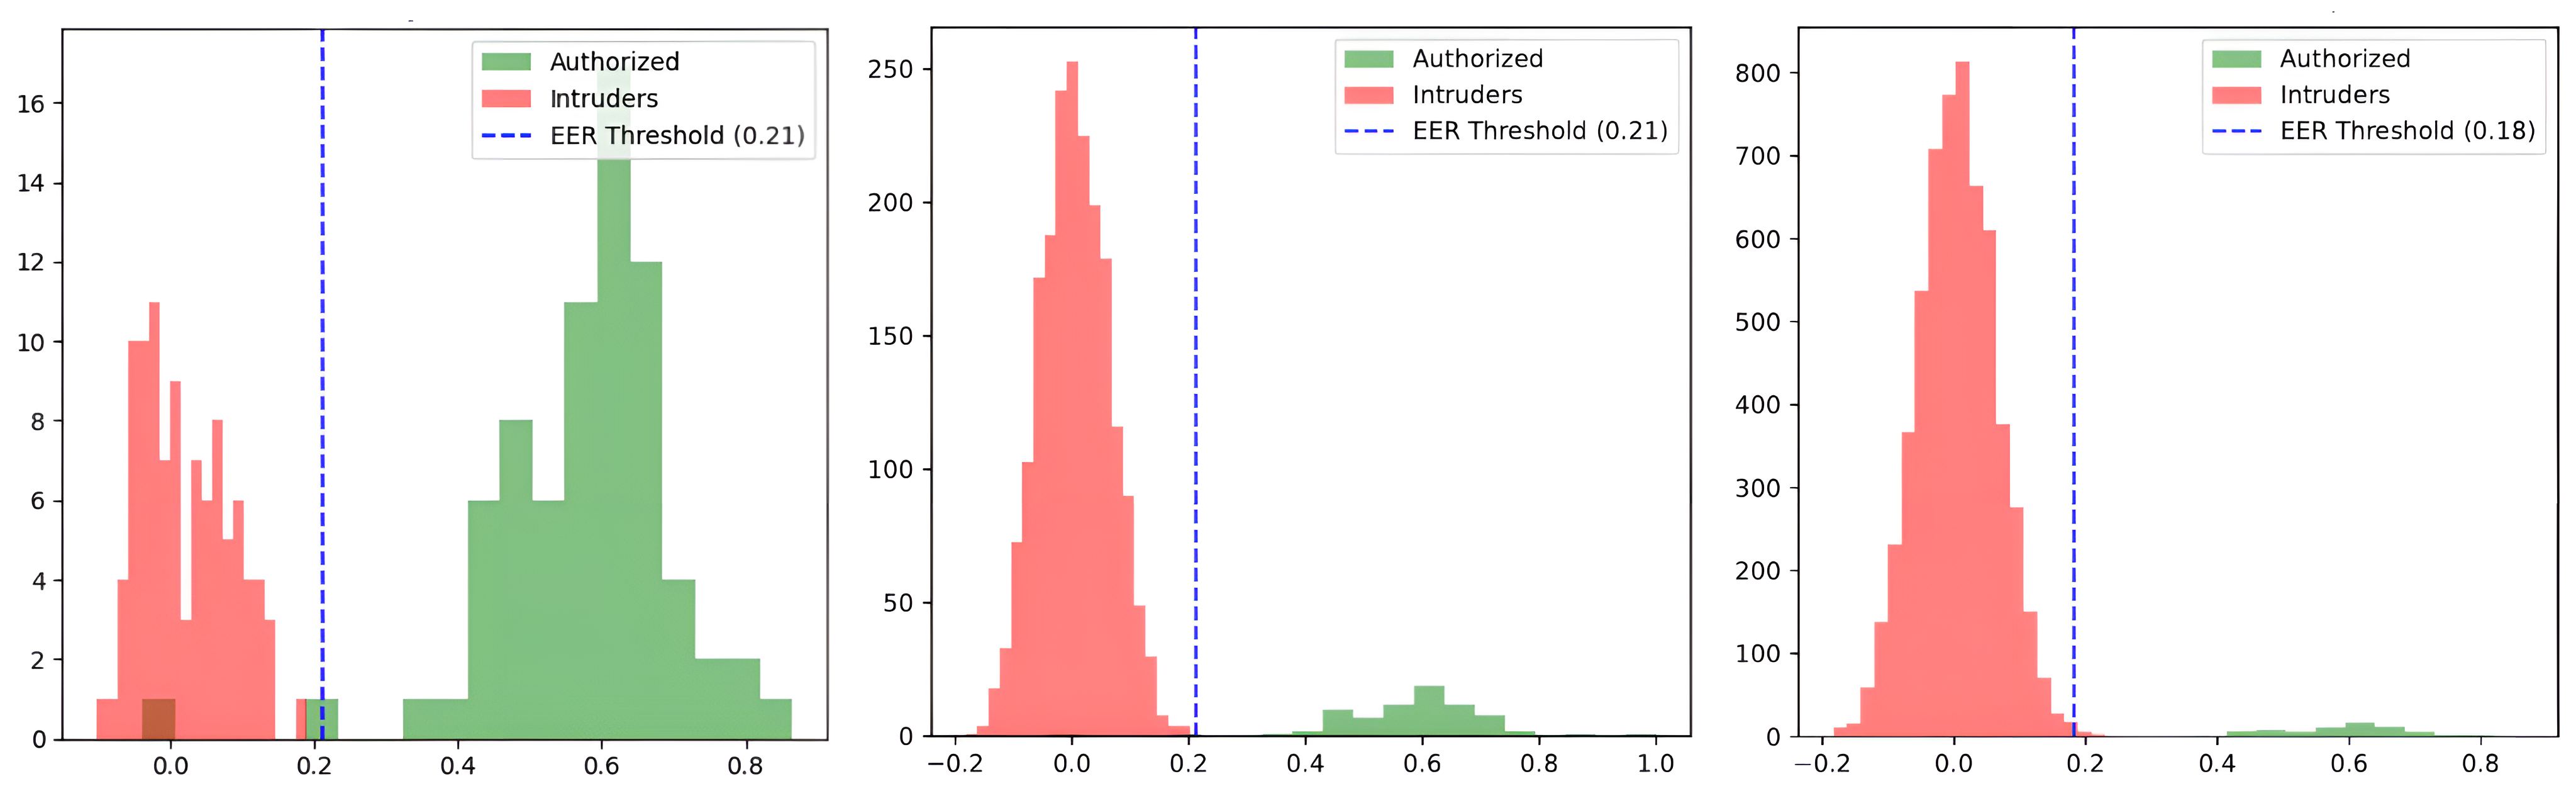
\includegraphics[width=0.94\textwidth]{fig_offline_eer}
\caption{Similarity scores of the enrolled operator against impostors, as the
negative set grows: 100 webcam images of other individuals, then $N=4{,}678$,
then the full $N=13{,}410$ including Labeled Faces in the
Wild~\cite{huang2008}. The dashed line is the equal-error threshold, which holds
at 0.21 until the negative set is enlarged and then settles at 0.18 at an equal
error rate of 0.32\%. The two populations stay separated throughout; what
Section~\ref{sec:identity} measures is what happens to that separation when the
imagery comes from the aircraft. Produced by I. Chaabeni outside this
repository, and recorded as external by the audit.}
\label{fig:offlineeer}
\end{figure*}

The embedding is characterised first in the manner conventional for the
component. A positive set of 76 images of the enrolled operator, mixing selfies,
webcam captures and standard photographs, was scored against a negative set
combining 100 webcam images of other individuals from a public face-detection
dataset with approximately 13{,}000 images from Labeled Faces in the
Wild~\cite{huang2008}. Against the 100-image negative set the two classes
separate perfectly, at an equal error rate of 0.0\%. Against the full combined
set of 13{,}410 the rate is 0.32\%, at an equal-error threshold of $\tau=0.18$.

That benchmark is not the operating point the aircraft runs at. The deployed gate
opens at $\tau_{\mathrm{on}}=0.55$, chosen for impostor margin rather than for
equal-error balance, so comparing the two figures directly confounds a change of
imagery with a change of threshold. Table~\ref{tab:frr} separates them by holding
the threshold fixed.

At the offline threshold, moving from curated stills to the aircraft's own video
raises false rejection from 0.32\% to 7.3\%, a factor of 23. H.264 compression,
motion blur, variable illumination and a moving camera are the obvious
candidates; a fourth is that the embedding is used outside the pipeline it was
trained in, on an unaligned crop from a different detector
(Section~\ref{sec:gate}). Which of the four dominates is not resolved here,
since separating them needs a capture that varies one at a time.
Raising the threshold to the deployed 0.55 raises it again to 35.1\%: the choice
of operating point costs more than the change of imagery does. The deployed gate
recovers part of that, since the Schmitt trigger of \eqref{eq:gate} holds
authorization through brief excursions below $\tau_{\mathrm{on}}$ and returns
19.3\% against 35.1\% for the same frames thresholded independently. Hysteresis
is worth 16 points of false rejection, measured on identical data.

On the ground, inside the working envelope established below, false rejection
is 16.7\% per frame and 9.2\% through the deployed gate over 2792 frames. Both
sit below the corresponding in-flight rates, which is the expected ordering:
flight is the harder condition.

\begin{figure}[t]
\centering
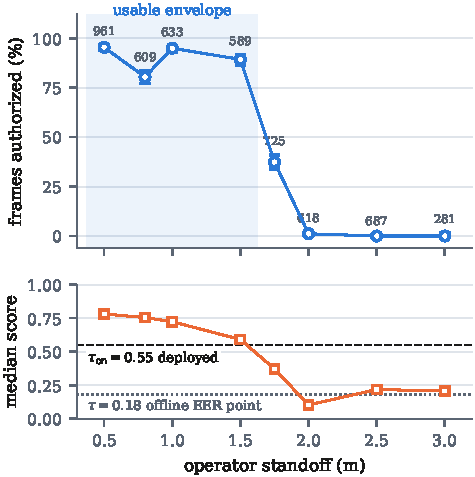
\includegraphics[width=0.92\columnwidth]{fig_envelope}
\caption{Authorization rate $\uparrow$ against operator standoff, frame counts
annotated, Wilson intervals. Below: median similarity against the two
thresholds.}
\label{fig:envelope}
\end{figure}

Figure~\ref{fig:envelope} reports authorization against declared standoff over a
cued ground sweep of 5{,}103 scored frames at eight marked distances. Between
0.5 and 1.5~m the gate admits 80--95\% of frames; at 1.75~m it admits 37\%, and
at 2.0~m and beyond essentially none. The usable envelope is therefore
0.5--1.5~m.

The same sweep calibrates the face-following standoff against the gate's. Over
the 4{,}861 frames at marks inside the envelope the median of $\sqrt{\rho_t}\,d$ is
0.258~m, with $\rho_t$ the face box as a fraction of frame area and $d$ the
declared distance. The follower's target $\rho^{\star}=0.075$
(Section~\ref{sec:facefollow}) therefore sits at 0.94~m, with a holding band of
0.90--1.00~m from its deadband, near the middle of the range the gate admits.
The offline benchmark cannot supply this, since it relates a control parameter
to a physical standoff through the deployed optics.

Beyond the envelope the failure changes character. Median apparent face size
falls with distance as far as 1.75~m and then rises again, from 132~px to 165,
211 and 210~px at 2.0, 2.5 and 3.0~m, which no receding face can do. Beyond
2.0~m the scores have mean 0.177 and standard deviation 0.082, statistically the
background population Section~\ref{sec:staleness} identifies at
$0.193\pm0.033$: the detector is returning false positives on the backdrop and
the gate is embedding them. Identity refuses them correctly, but arbitration is
still told a face is present --- the coupling of Section~\ref{sec:staleness}
reached through range rather than staleness.

\subsection{Stale Bounding Boxes in the Identity Path}
\label{sec:staleness}

The arbitration layer holds \texttt{face\_detected} true for 2~s across detection
gaps so mode selection does not flicker on a low-frame-rate stream. The identity
path initially reused this predicate, so once the operator's face leaves a
bounding box the system embeds whatever the box now contains.


\begin{figure}[t]
\centering
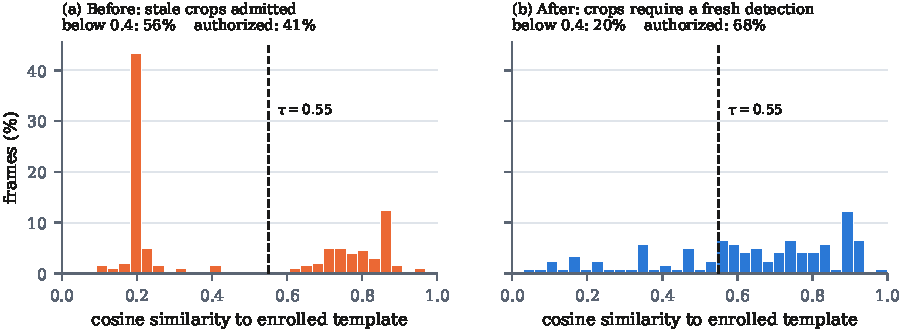
\includegraphics[width=0.86\columnwidth]{fig_score_distribution}
\caption{Cosine similarity to the enrolled template before and after restricting identity crops to fresh detections. The cluster near 0.19 in (a) is background embedded from a box the face had already left.}
\label{fig:scoredist}
\end{figure}

The resulting distribution (Figure~\ref{fig:scoredist}) is bimodal: a genuine
cluster at $0.770$ ($\sigma=0.109$) and a tighter one at $0.193$
($\sigma=0.033$) composed of background embeddings. A marginal operator would
give a unimodal distribution; two tight clusters indicate two distinct inputs.

Restricting identity crops to detections under 0.35~s old, and removing a
compounding second throttle, reduced the background cluster from 56\% to 20\% of
frames and raised the authorized fraction at $\tau=0.55$ from 41\% to 68\% over
matched runs. The clearest indicator is downstream: \texttt{search\_360}
decisions fell from 130 to 4 and \texttt{face} decisions rose from 72 to 82.
Prior to the correction the aircraft repeatedly concluded that no operator was
present while the operator stood within its field of view.

Arbitration requires a persistent signal and identity a fresh one, so a single
hold time cannot serve both. This is invisible to component-level testing,
since each component is individually correct.

\subsection{Authorization Hysteresis}
\label{sec:hysteresis}


Under a per-frame threshold, an operator scoring near $\tau$ produces alternating
authorized and unauthorized frames. The arbitration layer is designed to operate
over a stable signal, so this chatter is amplified into spurious mode changes and
refused commands, and the mode-level hysteresis operates on an already corrupted
input.

The mechanism is visible in the one failed trial. The operator raised a hand at
$t=2.08$~s, but it remained unauthorized while the score sat in the band around
$\tau$ and then fell through it (0.675, 0.479, 0.507, 0.513, 0.423, 0.414,
0.440, 0.455); preemption occurred only at $t=4.20$~s, against a 1.53~s median
over the 19 successful trials in the same arm. Replaying the trial's 15 recorded
scores through \eqref{eq:gate} yields 13 authorized frames rather than 5, and
preemption at 2.08~s, in the frame the hand first appeared.

In flight, over matched three-minute runs of repeated operator entry and exit
from the field of view, disabling authorization hysteresis raises the mode-switch
rate from 15.7 to 78.5 per minute, a factor of 5.0. Disabling the identity gate
entirely reduces it to 9.7, since any face then sustains tracking; this is the
stability cost of the gate rather than an improvement.

The latch can be inherited: if the operator departs while authorization is held,
an impostor may briefly be admitted. Measured against impostor score traces it
clears in a median of three detections, approximately 1.5~s, and in-trial
impostor authorization rose from 0.0\% to 5.6\% of frames while all 20 impostor
trials were still rejected. At $n=20$ the trial count does not resolve a small
increase in false acceptance, so the frame-level rate is the operative figure.

\subsection{Flight Behaviour and Deployment Constraints}
\label{sec:flightbehaviour}

Three further behaviours were measured in flight.

\emph{Search coverage.} Yaw telemetry puts the deployed sweep at a median
318\textdegree{} over 22 episodes, terminating at a median 19.9~s on
reacquisition. Its 28~s duration is set by the yaw rate: at the configured
$\approx$13\textdegree/s a full rotation requires 28~s, and the RC limit yields
only $\approx$43\textdegree/s. An earlier 5~s specification covered a median
60\textdegree{} for that reason, and no command produces a rotation in 5~s. The
rate is not raised because the sweep exists to detect a face, and faster
rotation blurs the frame enough that the detector fails on the operator it
passes.

\emph{Battery failsafe.} Stepping the threshold down after each activation
produced eleven consecutive automatic landings between 91\% and 21\% charge in
one 580~s flight; the deployed value is 15\%.

\emph{Radio environment.} Stream rate varied between 4 and 24~fps across 31 runs.
Battery charge does not explain it (pooled $r=-0.08$ across 31 runs, with the
sign reversing between sites); venue does. In a university building with dense access-point coverage a
ground test achieved 21.8~fps with no reconnections, whereas flight in the same
room on the same link gave 8.4~fps with 48 reconnections and SDK command timeouts
while airborne, including a failed emergency stop. At a domestic site the same
code achieved 19.7--22.3~fps with one reconnection. Motor interference, higher
current draw and a rotating antenna occur only in flight, so bench evaluation
does not expose this constraint.

\subsection{Reason-Only Language Model}
\label{sec:llm}

In one instrumented run the model was called 199 times, and because a reason
persists in the log until it changes, those calls populate 490 decision records.
Eleven of the 199 calls returned a timeout rather than a sentence, 5.5\% of
calls, which propagate to 35 of the 490 records, 7.1\% of records. Among the
calls that did return, the model produced statements contradicting the state
supplied to it: across all runs the verbatim low-battery sentence was emitted at
charges as high as 94\%, despite a system prompt forbidding invented battery
warnings, and the most frequent output was a restatement of the deterministic
reason string. Latency averaged 1766~ms with a 95th percentile of 4002~ms, at
the configured timeout. Each figure is one of the three properties
Section~\ref{sec:reasondesign} excluded the model from actuation for, measured:
the latency exceeds the command interval by two orders of magnitude, and a model
that invents a low-battery warning at 94\% charge is asserting a state the
telemetry contradicts.

% =====================================================================
\section{Discussion}

Three of the behaviours above share a structure, each arising between
components that were individually correct and individually characterised: the
stale crop from two of them sharing one temporal predicate
(Section~\ref{sec:staleness}), the authorization chatter from a correct
threshold feeding a correct state machine (Section~\ref{sec:hysteresis}), and
the spurious depth commands from a correct rule evaluated at an uncontrolled
rate (Section~\ref{sec:depth}). Section~\ref{sec:packing} is not of that kind:
there the estimator and the classifier both behave as specified and the fault is
in the specification, a vocabulary whose classes are separated by less than the
landmark estimator resolves, which no amount of correct composition repairs.
None of the four was exposed by component-level evaluation, nor by the scenario
validation of Section~\ref{sec:results} in which every trial passed, but
by per-frame logging of internal state, latency conditioned on the frames where
work occurred, and operational rates recorded alongside offline metrics. The
findings are properties of this implementation; the measurement practice that
produced them is not.

The experiments support a layer-separated reading of \method{IGate}: arbitration
requires a persistent signal and identity a fresh one, so the two cannot share a
temporal parameter, and arbitration-level hysteresis cannot repair a signal
already made unstable upstream. \method{IGate} therefore parameterises
authorization and arbitration separately rather than as one filter chain.

\subsection{What is Specific to the Platform}

The gap between a reported figure and a deployed one has a parallel in the
simulation-to-reality literature, where the mismatch is between a model of the
world and the world~\cite{aljalbout2025realitygap}; here both measurements are
taken on the same hardware and the mismatch is between two evaluation
protocols over the same component.

Only the absolute rates belong to this aircraft. A 19.3\% false rejection rate,
a 4--24~fps stream and a 0.5--1.5~m envelope follow from one rolling-shutter
camera, one H.264 encoder and one 2.4~GHz link, and better hardware moves all
three. Three other classes of finding do not move with it. A temporal predicate
shared between a layer that needs persistence and one that needs freshness is a
composition error a faster camera makes rarer without making correct
(Section~\ref{sec:staleness}); a vocabulary demanding more precision than the
perception stack delivers is a specification error repaired by redesigning the
vocabulary (Section~\ref{sec:packing}); and the measurement practice --
conditioning latency on the frames where a stage ran, deduplicating by sequence
number, reporting operational rates beside offline ones -- is what makes the
first two distinguishable at all.

\subsection{Limitations}
\label{sec:limitations}

The in-flight comparison suppresses actuation, so it does not measure the
closed loop in which a command moves the aircraft and changes the operator's
framing. The two arms are cued on different vocabularies, necessarily, so the
comparison is between deployed capabilities rather than classifiers on matched
input, and the operator cannot be blinded to the arm. The results characterise
one enrolled operator across four sessions; that depth is what made the
stale-crop and hysteresis findings visible, and extending the identity results
across operators is the natural next study. The evaluation addresses whether the
system performs as specified rather than how well an operator performs with it.
The gate establishes that an authorized operator is present, not that the
commanding hand is theirs: admission is a conjunction of two independent tests
and the perception path never binds hand to face
(Section~\ref{sec:gate}). Binding them through person detection is the most
valuable extension, and the released instrumentation suffices to quantify the
current exposure. The radio-environment result rests on two sites.

\section{Conclusion}

This paper proposed \method{IGate}, an identity-gated gesture control stack for
a low-cost indoor drone, and evaluated it through 270 logged trials of which 149
were flown. Every valid flight trial produced the specified behaviour.

The offline and operational figures disagree, and by how much depends on what
the component rests on. Gesture accuracy falls 0.997, 0.910, 0.783 across three
successively stricter protocols, almost entirely through the choice of split;
face verification operates at 19.3\% false rejection in flight against a 0.32\%
offline equal error rate, a gap that divides into the cost of the imagery and
the cost of an operating threshold three times the equal-error point. Flown
under a hover-locked cue at matched standoff the RBF-SVM reaches 0.850 and the
geometric rule 0.651, with 82\% of that gap on the depth channel, and expressing
depth as a pose rather than a motion takes FORWARD from 0.000 to 0.777 while
leaving BACK at 0.336, below what the landmark estimator resolves. Six
deployment behaviours were quantified from the logs and three corrected with
paired measurements. These results support reporting operational rates and
conditioned per-stage latency alongside offline benchmarks for systems of this
class.

\section*{Ethics, Data and Code Availability}

Face images of the operator were collected by the operator; public face datasets
were used only for offline evaluation. The enrolled embedding is held in volatile
memory for the session and is not persisted. The system implements no liveness
detection or anti-spoofing and is not a biometric security mechanism: its threat
model is prevention of accidental control by bystanders after enrolment. Indoor
flight used propeller guards, conservative command limits and manual supervision.
Implementation, instrumentation, all run logs and the table- and
figure-generation scripts will be released at
\url{https://github.com/Diyari-Fariq-M-salih/gesture-controlled-tello-drone}. The
authors thank the M2 Smart Aerospace and Autonomous Systems programme at
Universit\'e Paris-Saclay.

\balance
\bibliographystyle{IEEEtran}
\bibliography{references}

\end{document}
